\documentclass[11pt]{article}
\usepackage{graphicx}
\usepackage{amsthm}
\usepackage{latexsym}
\usepackage{amssymb}
\usepackage{amsmath}
\usepackage{listings}
\usepackage[usenames]{color}
\lstset{language=Java}
\usepackage{colortbl}
\definecolor{CommentColor}{rgb}{0,0.45,0.08}
\lstset{
    basicstyle=\ttfamily\tiny,
    keywordstyle=\color{blue},
    commentstyle=\color{CommentColor},
    tabsize=4
}
\newtheorem{theorem}{}
\newcommand{\ra}{\Rightarrow}
\renewcommand{\iff}{\Leftrightarrow}
\newcommand{\bt}{\textbf{T}}
\newcommand{\vc}[1]{\mathbf{#1}}
\newcommand{\dotp}[2]{\vc{#1} \cdot \vc{#2}}

\bigskip
\author{Priyananda Shenoy (shenoy@cs.wisc.edu)}
\title{	CS 540 Fall 2008 Homework 4}
\setlength{\parindent}{0in}

\begin{document}
\maketitle
\begin{center}
	Late Days used: \underline{0}
\end{center}

\newpage

1. [a] is linearly separable, hence is computable by a 1-layer perceptron.
[b] is always false, hence is trivially linearly separable. As we saw in class,
the XOR function is not linearly separable. Since the negation of a function is
just flipping the labels, [c] is also not linearly separable. Parity is the
same as XNOR, hence [d] is also not linearly separable. Hence [c] and [d] have
no single-layer perceptrons.

\begin{center} 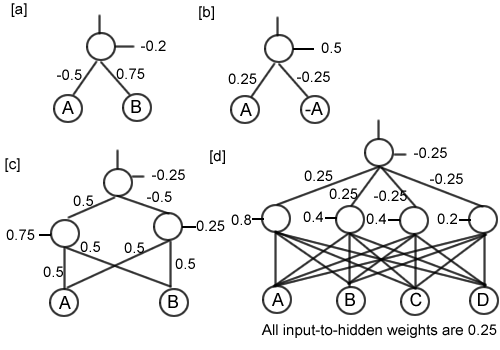
\includegraphics[width=350px,height=225px]{1.png} \end{center}

2. 

[a] \begin{center} 
\includegraphics[width=200px,height=150px]{2.png} \end{center}

[b] The sigmoid function is defined as
\[ \sigma(\vc{x}) = \frac{1}{1 + e^{-\dotp{w}{x}}}. \]
For hidden gate H1,
\begin{align*}
	\dotp{w}{x} &= (0.5)(A) + (0.5)(B) + (0.5)(C) + (0.2)(-1) \\
		&= (0.5)(0.3) + (0.5)(0.8) + (0.5)(0.1) - 0.2 \\
		&= 0.4 \\
	h_1 &= \sigma(0.4) = \frac{1}{1 + e^{-0.4}} = \frac{1}{1 + 0.67} = 0.5987.
\end{align*}

For hidden gate H2,
\begin{align*}
	\dotp{w}{x} &= (-0.2)(A) + (-0.2)(B) + (-0.2)(C) + (0.2)(-1) \\
		&= - (0.2)(0.3) - (0.2)(0.8) - (0.2)(0.1) - 0.2 \\
		&= - 0.44 \\
	h_2 &= \sigma(-0.44) = \frac{1}{1 + e^{0.44}} = \frac{1}{1 + 1.553} = 0.3917.
\end{align*}
	
The expected output with these set of weights is,
\begin{align*}
	\dotp{w}{x} &= (0.5)(h_1) + (-0.2)(h_2) + (0.2)(-1) \\
		&= (0.5)(.5987) - (0.2)(.3917) - 0.2 \\
		&= 0.021 \\
	d &= \sigma(0.021) = \frac{1}{1 + e^{-0.021}} = \frac{1}{1 + 1.9792} = 0.5052.
\end{align*}

The error at the output is
\begin{align*}
	\Delta &= \sigma'(\{h_1,h_2,-1\}) \cdot (D - d) \\
	\sigma'(\vc{x}) &= \sigma(\vc{x})(1 - \sigma(\vc{x})) \\
		&= (0.5052)(1 - 0.5052) = 0.25 \\
	\Delta &= (0.25)(1 - 0.5052) = 0.1237
\end{align*}

Backpropogating error to H1,
\begin{align*}
	\Delta_{h1}  &= \sigma'(h_1) W_{H1D} \Delta \\
	\sigma'(h_1) &= 0.5987 ( 1 - 0.5987) = 0.2402 \\
	\Delta_{h1}  &= 0.2402 \cdot 0.5 \cdot 0.1237 = 0.0149 \\
	W_{H1D} &= W_{H1D} + \alpha h_1 \Delta_{h1} \\
		&= 0.5 + 0.3 \cdot 0.5987 \cdot 0.0149 \\
		&= 0.5027
\end{align*}

Backpropogating error to bias node,
\begin{align*}
	\Delta_{d'}  &= \sigma'(-1) W_{d'D} \Delta \\
	\sigma'(-1)  &= .2689 ( 1 - .2689 ) = 0.1966 \\
	\Delta_{d'}  &= 0.1966 \cdot 0.2 \cdot 0.1237 = 0.0049 \\
	W_{d'D} 		 &= 0.2 + 0.3 \cdot 0.0049 \cdot -1 = 0.1985
\end{align*}

Backpropogating error to H2,
\begin{align*}
	\Delta_{h2}  &= \sigma'(h_2) W_{H2D} \Delta \\
	\sigma'(h_2) &= 0.3917 ( 1 - 0.3917) = 0.2383 \\
	\Delta_{h2}  &= 0.2383 \cdot -0.2 \cdot 0.1237 = -0.0059 \\
	W_{H2D} &= W_{H2D} + \alpha h_2 \Delta_{h2} \\
		&= -0.2 + 0.3 \cdot 0.3917 \cdot -0.0059 = -2.0007 \\
		&= 0.5027
\end{align*}

Backpropogating error to A,
\begin{align*}
	\Delta_{A} &= \sigma'(A) ( W_{AH1} \Delta_{h1}  + W_{AH2} \Delta_{h2} ) \\
						 &= 0.2445 ( 0.5 \cdot 0.0149 - 0.2 \cdot 0.0049) \\
						 &= 0.00158 \\
	W_{AH1} 	 &= 0.5 + 0.3 \cdot 0.3 \cdot 0.00158 \\
						 &= 0.5001 \\
	W_{AH2}		 &= -0.2 + .3 \cdot 0.3 \cdot 0.00158 \\
						 &= -0.1999
\end{align*}

Backpropogating error to B,
\begin{align*}
	\Delta_{B} &= \sigma'(B) ( W_{BH1} \Delta_{h1}  + W_{BH2} \Delta_{h2} ) \\
						 &= 0.2139 ( 0.5 \cdot 0.0149 - 0.2 \cdot 0.0049) \\
						 &= 0.00138 \\
	W_{BH1} 	 &= 0.5 + 0.3 \cdot 0.3 \cdot 0.00138 \\
						 &= 0.5001 \\
	W_{BH2}		 &= -0.2 + .3 \cdot 0.3 \cdot 0.00138 \\
						 &= 0.1999
\end{align*}

Backpropogating error to C,
\begin{align*}
	\Delta_{C} &= \sigma'(C) ( W_{CH1} \Delta_{h1}  + W_{CH2} \Delta_{h2} ) \\
						 &= 0.2494 ( 0.5 \cdot 0.0149 - 0.2 \cdot 0.0049) \\
						 &= 0.00161 \\
	W_{CH1} 	 &= 0.5 + 0.3 \cdot 0.3 \cdot 0.00161 \\
						 &= 0.5001 \\
	W_{CH2}		 &= -0.2 + .3 \cdot 0.3 \cdot 0.00161 \\
						 &= 0.1986
\end{align*}

3. The XOR function over the $\{1,-1\}$ domain is defined as follows. We will use the map
$(x_1,x_2) \mapsto (x_1,x_1x_2)$ to linearly separate the XOR function.

\begin{center}
\begin{tabular}{|c|c|c|c|}
\hline
$x_1$ & $x_2$ & $x_1x_2$ & $x_1 \;XOR\; x_2$ \\
\hline
-1  & -1	&  1		 & -1 \\
-1  &  1	& -1		 &  1 \\
1   & -1	& -1		 &  1 \\
1   &  1	&  1		 & -1 \\
\hline
\end{tabular}
\end{center}

\begin{center} 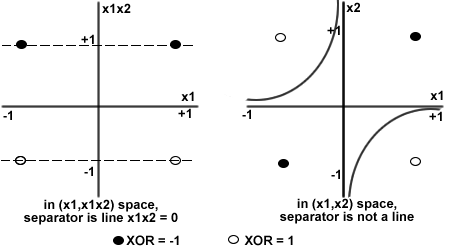
\includegraphics[width=350px,height=225px]{3.png} \end{center}

Any line $x_1x_2 = c, -1 \leq c \leq +1$ is a separator in the transformed space.
The maximal margin separator is the line $x_1x_2 = 0$, which has margin (1+1) = 2.
The separator doesn't remain a line in $(x_1,x_2)$ space. The separator $x_1x_2 = c$
becomes the hyperbola $x_2 = \frac{c}{x_1}$ in euclidean space, with the degenerate
hyperbola $x_1x_2 = 0$ being the maximal margin separator.

\renewcommand{\labelenumi}{\arabic{enumi}.}
\renewcommand{\labelenumii}{[\alph{enumii}]}

Question 4. Part 1
\begin{enumerate}
	\item
		\begin{enumerate} 
			\item 1.19 seconds.
			\item 63.35\% of examples.
			\item Confusion matrix
			\begin{tabular}{|c|c|l|}
			\hline
			  a  & b  &  classified as \\
			\hline
		 		81 & 48 &  a = face \\
		 		44 & 78 &  b = non-face \\
		 	\hline
		 	\end{tabular}
		 	\item The SVM had errors in both directions(i.e. classifying faces as non-faces and vice versa).
		\end{enumerate}
 	
 	\item
 		\begin{enumerate} 
			\item 2.48 seconds.
			\item 65.74\% of examples.
			\item The results improved by $\approx 2\%$. The `exponent' option controls the exponent of
			the polynomial kernel. The improvement shows that while the data is not linearly separable,
			the data when mapped to some space through a quadratic transformation, the separation
			increases.
		\end{enumerate}
	
	\item
 		\begin{enumerate} 
			\item 73.31\% of examples.
			\item There was a significant difference in the accuracy using RBF instead of polynomial
			kernel. This shows that the data is not quadratically separable, but separation
			increases if a radial basis function is used to transform the feature space.
		\end{enumerate}
\end{enumerate}

Part 2
\begin{enumerate}
	\item
		\begin{enumerate}
			\item
			\begin{tabular}{|c|c|c|c|}
				\hline
					Learning Rate & Hidden Layers & Training Time & Success Percentage \\
				\hline
					0.1 &  5	&	7.09s & 64.54\%\\
					0.1 & 10	&	12.56s& 63.74\%\\
					0.1 & 20	&	23.81s& 64.14\%\\
					0.3 &  5	&	6.95s & 67.93\%\\
					0.3 & 10	&	11.91s& 66.93\%\\
					0.3 & 20	&	22.39s& 68.13\%\\
				\hline       
			\end{tabular}
			
			\item The most successful network for this data was learnt using
			 learning rate = 0.3 and 20 hidden layers.	For a given learning rate, increasing
			 the number of hidden layers beyond a threshold  results in 
			 a network which overfits the training data. For a fixed time bound on
			 training time, a faster learning rate results in more accurate networks.
		\end{enumerate}
		
		\item
			\begin{enumerate}
				\item
					\begin{tabular}{|c|c|c|}
					\hline
						Learning rate & Time to train & Percentage correct \\
					\hline
						0.1 & 38.12s & 64.94\% \\
						0.3 & 36.69s & 67.33\% \\
					\hline
					\end{tabular}
					
				\item With the same learning rate (0.3) and hidden layers(10), increasing the
				training time from 100 to 300 increased the success percentage from 66.93\% to
				67.33\%. This is not always guaranteed to increase, since past a certain
				threshold the network will begin to overfit the examples, and might do worse
				on the testing data.
				
				\item With training time set to 300, hidden layers to 5, learning rate to 0.3,
				we get a success rate of 66.14\% instead of 67.93\% when the training time
				was 100. So in this case extra training time made it worse.
			\end{enumerate}
			
		\item
			\begin{enumerate}
				\item Time: 28.27s, Success percentage: 67.73\%
				\item The epochs required by each fold were approximately \{80,52,500,92,77\}. The
				third fold reached the limit and stopped. The number of epochs are distributed
				widely, as they depend on the training set.
				\item Keeping hidden layers 10 and learning rate 0.3, the accuracies for different
				training times are \{ 100 = 66.93\% , 300 = 67.33\% , 500 = 67.73\% \}. So in
				this case training time did help in improving accuracy.
				\item NO ANSWER
			\end{enumerate}	
		
		\item
			\begin{enumerate}
				\item The following parameters were kept constant: hidden layers = 5, training time = 100,
					validation set size = 10, validation threshold = 20. The parameter 'Learning rate'
					varied in the range $\{0.1,0.2,\cdots,1.0\}$.
				
				\item For a fixed training time, the learning rate can affect the success percentage in
				two ways. If the learning rate is too small, the learning algorithm makes slow
				progress and doesn't reach the desired accuracy within the training time. With a large
				learning rate, the weights fluctuate a lot, and may not converge to a fixed value.
				There is an ``optimal'' learning rate at which the two factors give the best result.
					
				\item
						\begin{tabular}{|c|c|c|c|c|c|}
							\hline
								$\alpha$& 0.1 	 & 0.2   & 0.3   & 0.4 	 & 0.5 	 \\
							\hline
								\%		  & 61.35  & 64.14 & 63.34 & 66.14 & 63.75 \\
							\hline
							\hline
								$\alpha$& 0.6 	 & 0.7 	 & 0.8 	 & 0.9   & 1.0   \\
							\hline
								\%		  &	70.52 & 64.54 & 66.14 & 69.32 & 64.54  \\
							\hline
						\end{tabular}
				
				\item Graph\\
					
					\begin{center} 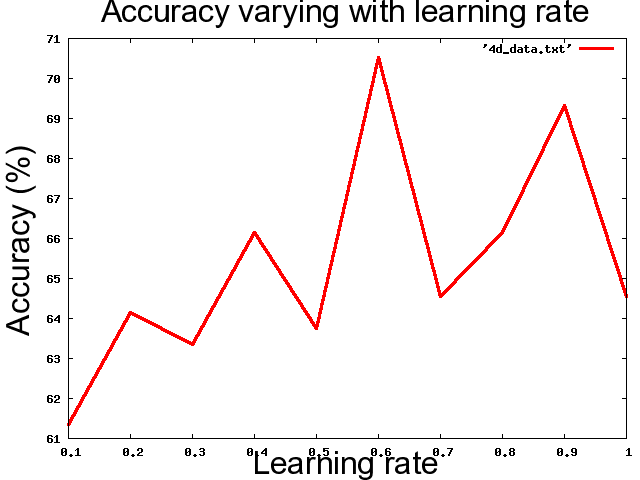
\includegraphics[width=200px,height=200px]{4d.png} \end{center}
				
				\item For the given training set, the best learning rate is 0.6.
			\end{enumerate}
\end{enumerate}


Question 5.


[a] The weights were $w_0 = 1.0, w_1 = 0.0, w_2 = 1.0$, where $w_0$ is the bias weight.

[b] The line $x_2 = 1.0$ is the decision boundary. The half-space defined by the
inequality $x_2 > 1.0$ gets the label `1' and the other half-space gets the label `0'.

\begin{center} 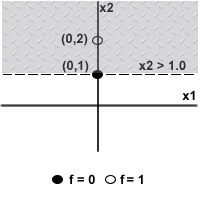
\includegraphics[width=150px,height=150px]{5.png} \end{center}

[c] With $\alpha = 0$, the algorithm never terminates. With any other learning rate,
the algorithm will eventually find the same result, but will differ in number of
iterations. In this small example, changing $\alpha$ didn't change the number of
interations. Also different $\alpha$ values give rise to different weights all
of which represent the same line.

[d] Weka classifies the data using the line $1 * x_2 - 1.5 > 0$. This is parallel
to the line which was found using our program.

\begin{center} 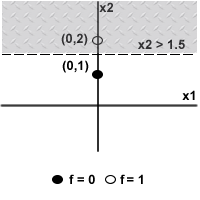
\includegraphics[width=150px,height=150px]{5d.png} \end{center}

[e] The example $(x_1 = 0, x_2 = 0, output = 1)$ makes the learning algorithm run
indefinitely since the data is now not linearly separable.

\end{document}